\documentclass[10pt, a5paper]{article}
\usepackage{pdfpages}
\usepackage{parallel}
\usepackage[T2A]{fontenc}
\usepackage{ucs}
\usepackage[utf8x]{inputenc}
\usepackage[polish,english,russian]{babel}
\usepackage{hyperref}
\usepackage{rotating}
\usepackage[inner=2cm,top=1.8cm,outer=2cm,bottom=2.3cm,nohead]{geometry}
\usepackage{listings}
\usepackage{graphicx}
\usepackage{wrapfig}
\usepackage{longtable}
\usepackage{indentfirst}
\usepackage{array}
\newcolumntype{P}[1]{>{\raggedright\arraybackslash}p{#1}}
\frenchspacing
\usepackage{fixltx2e} %text sub- and superscripts
\usepackage{icomma} % коскі ў матэматычным рэжыме
\PreloadUnicodePage{4}

\newcommand{\longpage}{\enlargethispage{\baselineskip}}
\newcommand{\shortpage}{\enlargethispage{-\baselineskip}}

\def\switchlang#1{\expandafter\csname switchlang#1\endcsname}
\def\switchlangbe{
\let\saverefname=\refname%
\def\refname{Літаратура}%
\def\figurename{Іл.}%
}
\def\switchlangen{
\let\saverefname=\refname%
\def\refname{References}%
\def\figurename{Fig.}%
}
\def\switchlangru{
\let\saverefname=\refname%
\let\savefigurename=\figurename%
\def\refname{Литература}%
\def\figurename{Рис.}%
}

\hyphenation{admi-ni-stra-tive}
\hyphenation{ex-pe-ri-ence}
\hyphenation{fle-xi-bi-li-ty}
\hyphenation{Py-thon}
\hyphenation{ma-the-ma-ti-cal}
\hyphenation{re-ported}
\hyphenation{imp-le-menta-tions}
\hyphenation{pro-vides}
\hyphenation{en-gi-neering}
\hyphenation{com-pa-ti-bi-li-ty}
\hyphenation{im-pos-sible}
\hyphenation{desk-top}
\hyphenation{elec-tro-nic}
\hyphenation{com-pa-ny}
\hyphenation{de-ve-lop-ment}
\hyphenation{de-ve-loping}
\hyphenation{de-ve-lop}
\hyphenation{da-ta-ba-se}
\hyphenation{plat-forms}
\hyphenation{or-ga-ni-za-tion}
\hyphenation{pro-gramming}
\hyphenation{in-stru-ments}
\hyphenation{Li-nux}
\hyphenation{sour-ce}
\hyphenation{en-vi-ron-ment}
\hyphenation{Te-le-pathy}
\hyphenation{Li-nux-ov-ka}
\hyphenation{Open-BSD}
\hyphenation{Free-BSD}
\hyphenation{men-ti-on-ed}
\hyphenation{app-li-ca-tion}

\def\progref!#1!{\texttt{#1}}
\renewcommand{\arraystretch}{2} %Іначай формулы ў матрыцы зліпаюцца з лініямі
\usepackage{array}

\def\interview #1 (#2), #3, #4, #5\par{

\section[#1, #3, #4]{#1 -- #3, #4}
\def\qname{LVEE}
\def\aname{#1}
\def\q ##1\par{{\noindent \bf \qname: ##1 }\par}
\def\a{{\noindent \bf \aname: } \def\qname{L}\def\aname{#2}}
}

\def\interview* #1 (#2), #3, #4, #5\par{

\section*{#1\\{\small\rm #3, #4. #5}}

\def\qname{LVEE}
\def\aname{#1}
\def\q ##1\par{{\noindent \bf \qname: ##1 }\par}
\def\a{{\noindent \bf \aname: } \def\qname{L}\def\aname{#2}}
}

\begin{document}
\title{Создание пакетов программной поддержки для процессоров собственной разработки}
\author{Роман Ставцев, Москва, Russian Federation\footnote{\url{lefty@mail.ru}, \url{http://lvee.org/ru/abstracts/302}}}
\maketitle
\begin{abstract}
The software development kit creating process for our own processors.
\end{abstract}
АО <<Байкал Электроникс>> фаблесс-компания специализируется на проектировании систем на кристалле (СнК) и интегральных микросхем. Основной продукцией является СнК \textbf{BE-T1000} и \textbf{BE-M1000}. Процессоры Baikal производятся на фабрике компании TSMC. Вспомогательной продукцией является программные пакеты (Software Development Kit, \textbf{SDK}) и оценочные платы.

Микропроцессор \textbf{BE-T1000}, другое название Байкал-Т1 относится к типу Система-на-кристале. Микропроцессор содержит два ядра MIPS32r5 P5600 Warrior.

\begin{center}
\begin{figure}[h!]
  \centering
  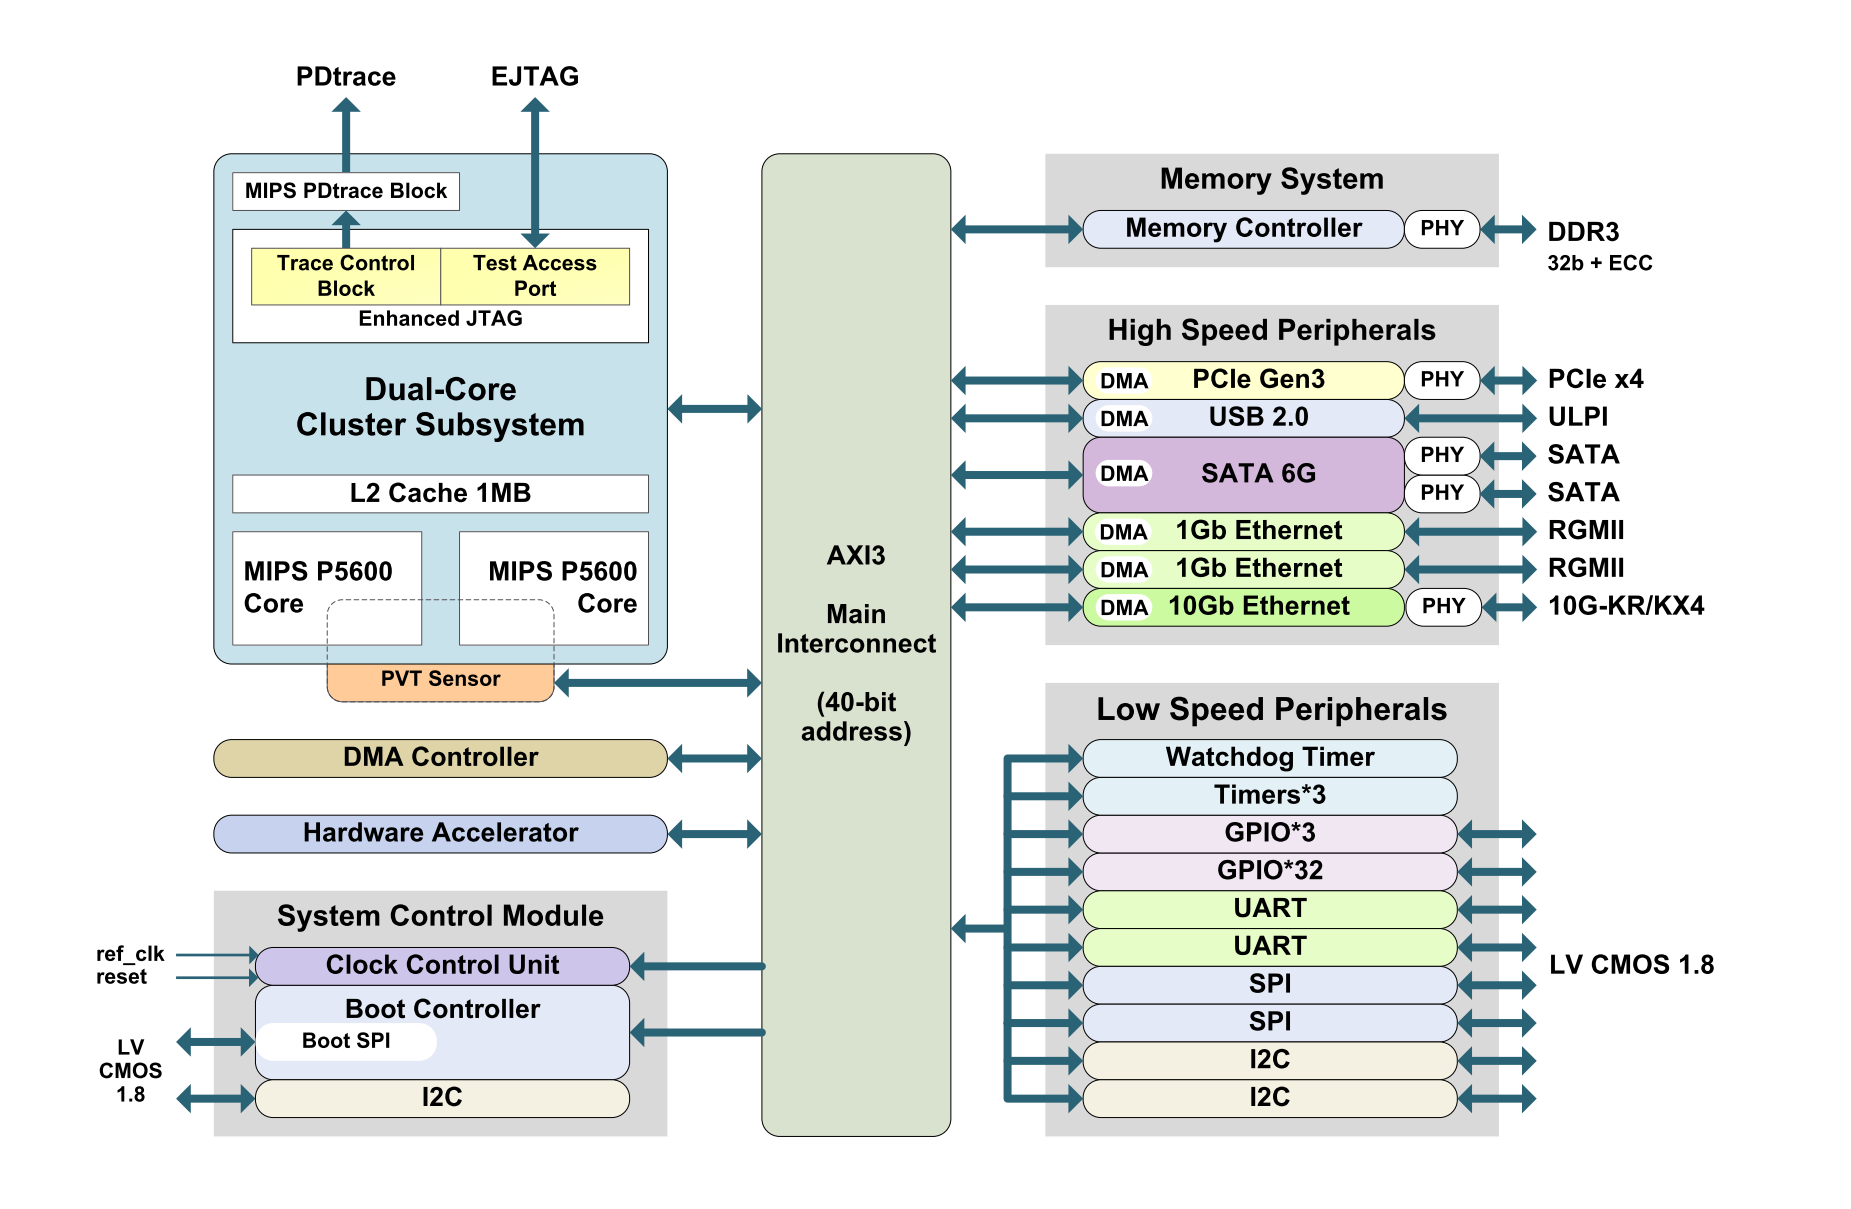
\includegraphics[width=10cm]{Stavtsev1}  
  \label{stavtsev:fig1}
\end{figure}
\end{center} 

Перечислим некоторые технические характеристики:

\begin{itemize}
  \item 2 ядра P5600 MIPS 32 r5, максимальная частота до 1,2 ГГц
  \item Кэш L2 1 Мбайт
  \item Контроллер памяти DDR3-1600
  \item Энергопотребление не более 5 Вт
*Технологический процесс 28 нм
\end{itemize}

Интегрированные интерфейсы:

\begin{itemize}
  \item 1 порт 10 Gb Ethernet
  \item 2 порта 1 Gb Ethernet
  \item контроллер PCIe Gen.3
  \item 2 порта SATA 3.0
  \item USB 2.0
\end{itemize}

Микропроцессор \textbf{BE---M1000}, другое название Байкал-M1 относится к типу Система-на-кристале.

\begin{center}
\begin{figure}[h!]
  \centering
  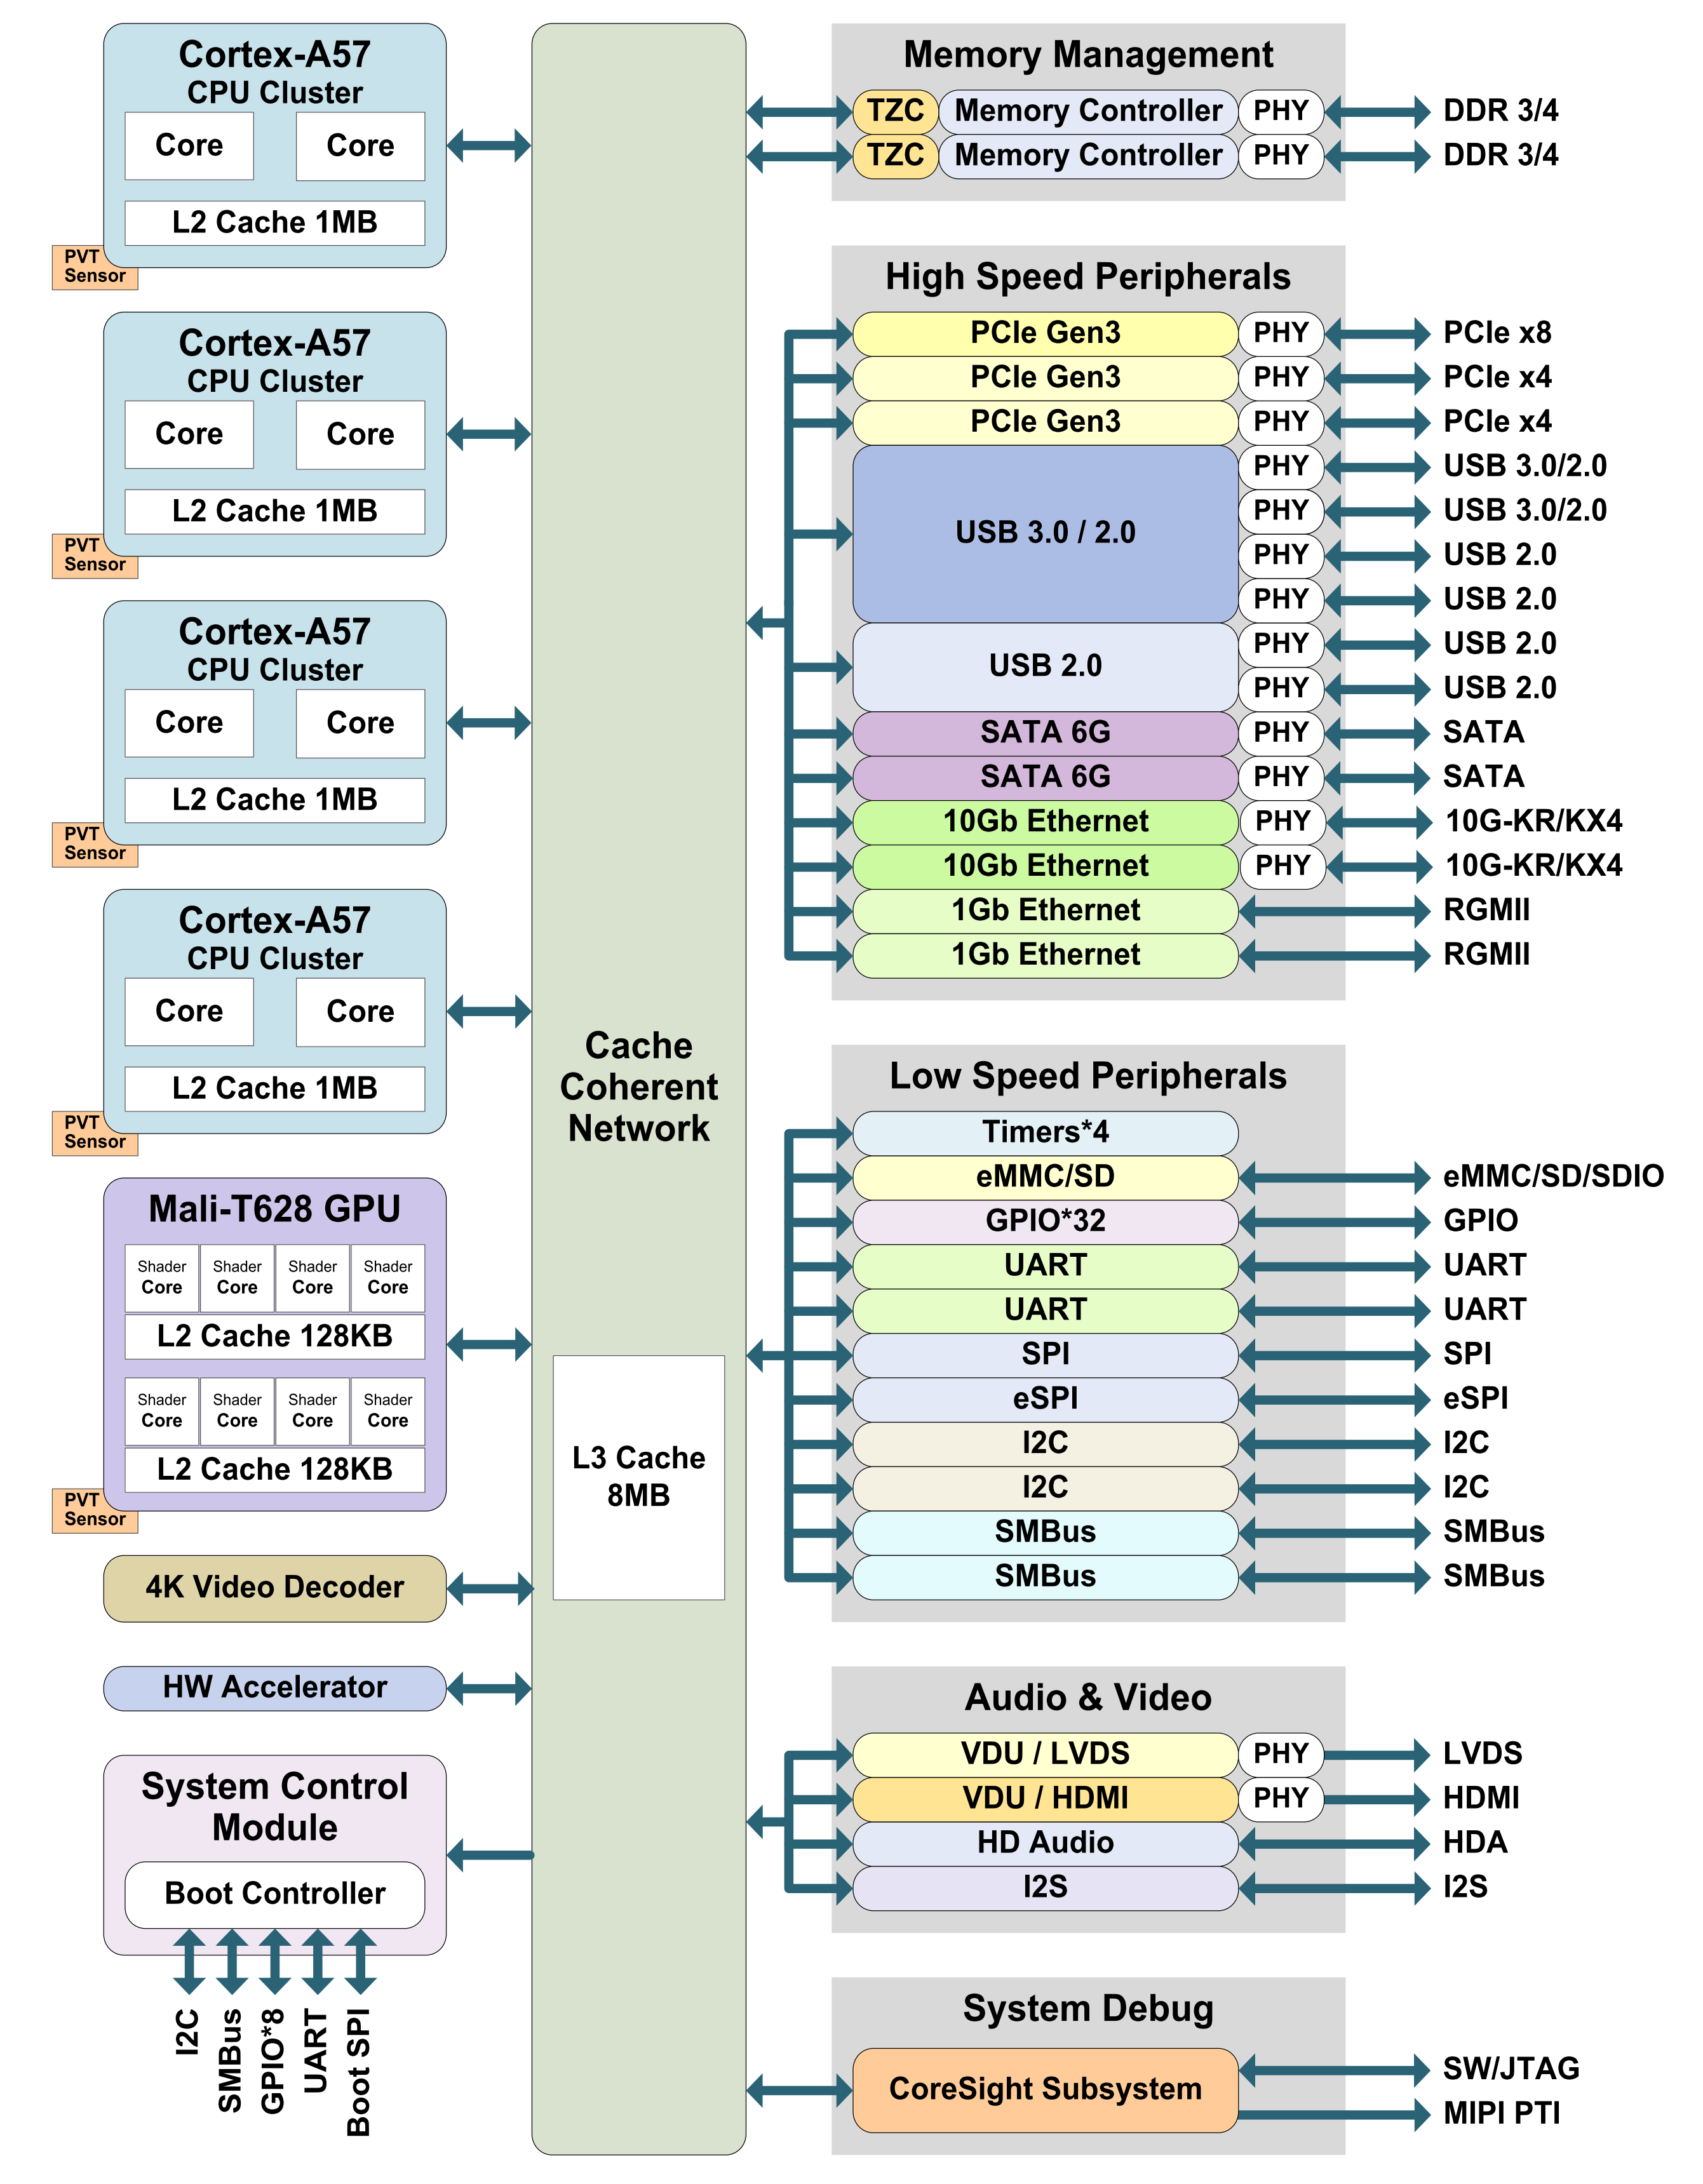
\includegraphics[width=10cm]{Stavtsev2}  
  \label{stavtsev:fig2}
\end{figure}
\end{center} 

Перечислим некоторые технические характеристики:

\begin{itemize}
  \item 4 кластера по 2 ядра ARM Cortex-A57, максимальная частота до 1,5ГГц
  \item Кэш L2 объемом 1 Мбайт на кластер
  \item Когерентный кэш L3 объемом 8 Мбайт
  \item 2 контроллера памяти DDR4-2400
  \item Графический процессор ARM Mail-T628 с поддержкой кэш L2 128 Кбайт на кластер
  \item 2 видеоконтроллера с поддержкой LVDS и HDMI2.0 интерфейсов
  \item Аппаратный 4K видео-декодер
  \item Аудио-подсистема HDAudio
  \item Подсистема управления загрузкой
  \item Технологический процесс 28 нм
  \item Корпус FCBGA 1521
\end{itemize}

Интегрированные интерфейсы:

\begin{itemize}
  \item 3 контроллера PCIe Gen3 (x8/x4/x4)
  \item 2 контроллера SATA 6G
  \item 2 контроллера XGb Ethernet
  \item 2 контроллера 1Gb Ethernet
  \item 2 контроллера USB 3.0/2.0 6 портов
\end{itemize}

Низкоскоростная периферия:

\begin{itemize}
  \item eMMC/SD/SDIO
  \item SPI/eSPI
  \item SMBus
  \item GPIO32
  \item UART
\end{itemize}

Программные пакеты \textbf{SDK} (Software Development Kit) для процессоров семейства Baikal, концентрируется на простоте установки и использования, предоставляя при этом необходимы инструментарий. В большей части SDK опирается на свободное программное обеспечение. Для каждого типа СнК выпускается свой SDK. SDK для BE-T1000 был основан на наборе собственных сборочных скриптов. Такой подход позволил создать автономную систему с минимумом зависимостей. Однако имеются и существенные ограничения в нашем решении, основное сложность создания изменяемых сборок с пользовательскими приложениями. При разработке SDK для BE-M1000 мы сохранили прежний принцип построения, понимая и принимая все плюсы и минусы такого решения.

Рассмотрим схожие компоненты SDK. В состав SDK входят средства разработки программ для целевого процессора, средства отладки, полный набор исходных кодов, комплект поддержки для отладочных/оценочных плат (BFK), образ встраиваемой операционной системы на основе ядра Linux и набора busybox, средства автоматизации сборки различных образов и прошивок для устройств на процессорах семейства Baikal.

Состав SDK выглядит следующим образом:

\begin{itemize}
  \item Загрузчик
  \item Ядро Linux
  \item Образ initrd встраиваемой ОС на основе пакета busybox
  \item Образ initramfs для запуска <<больших>> дистрибутивов ОС Linux
  \item Прошивка для загрузочной флеш-памяти
  \item Образ файловой системы для эмулятора QEMU
  \item Скрипты автоматизации сборки
  \item Тулчейн
  \item Вспомогательные утилиты
  \item Программный эмулятор
  \item Скрипты поддержки/автоматизации для эмулятора
  \item Исходные коды
\end{itemize}

Основные компоненты немного подробнее.

\subsection*{Загрузчик}

Мы используем модифицированную версию загрузчика U-BOOT для BE-T1000.
Начинали с U-BOOT v2014.10
Мы используем для BE-M1000 UEFI tianocore основанный на <<UEFI Development Kit>> UDK2017.

\subsection*{Ядро Linux}

для BE-T1000 были внесены дополнения в следующие ветки ядра Linux:
\begin{itemize}
\item 3.19.xx --- не поддерживается
\item 4.4.xx --- активно поддерживается (https://github.com/baikalelectronics/Linux-kernel.4.4.xx)
\item 5.2 --- в разработке
\end{itemize}
для BE-M1000 были внесены дополнения в следующие ветки ядра Linux
\begin{itemize}
\item 4.9.180 --- в разработке
\end{itemize}

\subsection*{Тулчейн}

Пакет средств кросс-компиляции на основе GNU gcc, binutils и т.д.
\begin{itemize}
\item gcc–8.3.0, binutils–2.32 (для BE-T1000, SDK-4.18)
\item gcc 6.3.0, binutils 2.28 (для BE-M1000)
\end{itemize}
Средства отладки (gdb)
\begin{itemize}
\item gdb–8.2.1 (для BE-T1000, SDK-4.18)
\item gdb 7.12.1 (для BE-M1000)
\end{itemize}
Предсобранные исполнимые файлы и библиотеки (sysroot) на основе glibc
\begin{itemize}
\item glibc–2.29 (для BE-T1000, SDK-4.18)
\item glibc 2.25 (для BE-M1000)
\end{itemize}

\end{document}
